\documentclass[12pt,a4paper,margin=1in]{report}
\usepackage[utf8]{inputenc}
\usepackage{amsmath}
\usepackage{amsfonts}
\usepackage{amssymb}
\usepackage{graphicx}
\usepackage{braket}
\usepackage{natbib}
\usepackage{tikz}
\usetikzlibrary{positioning}
\usetikzlibrary{shapes,arrows}
\usepackage{bm}
\usepackage[toc,page]{appendix}
\pagenumbering{arabic}
\linespread{1.3}


\tikzstyle{decision} = [ellipse, minimum width=1.5cm, minimum height=1cm, text centered, draw=black, fill=green!30]

\tikzstyle{block} = [rectangle, draw, fill=blue!20, 
    text width=6em, text centered, rounded corners, minimum height=4em]

\tikzstyle{end} = [rectangle, draw, fill=yellow!20, 
    text width=6em, text centered, rounded corners, minimum height=4em]

\tikzstyle{prelim} = [rectangle, draw, fill=red!20, 
    text width=6em, text centered, rounded corners, minimum height=4em]

\tikzstyle{arrow} = [thin,->,>=stealth]



\begin{document}
\chapter{Simulation Pipeline}
In this chapter the simulation of a hyperfine spectrum measured at TRIUMF is described in detail. $\S$\ref{pip} includes little more than a graphical representation of the algorithm followed. Each subsequent section is dedicated to an individual step in the algorithm, detailing the logic and computations required at that step. 

\begin{figure}[h]

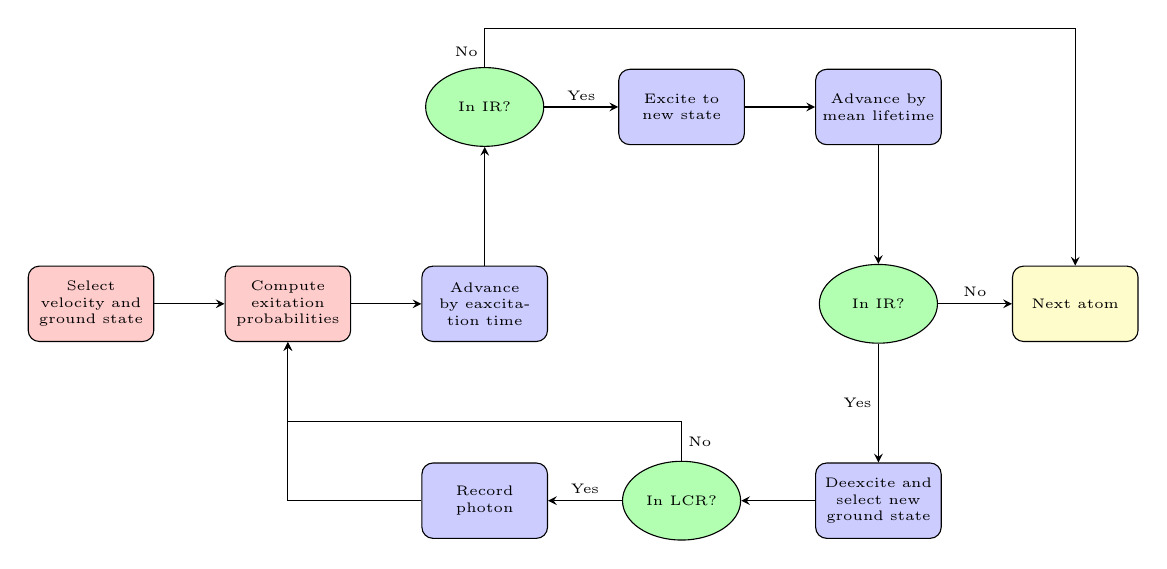
\begin{tikzpicture}[node distance = 2.5cm]
\tiny

\node (props) [prelim] {Select velocity and ground state};
\node (exprobs) [prelim, right of=props] {Compute exitation probabilities};
\node (Adv_exc) [block, right of=exprobs] {Advance by eaxcitation time};
\node (IR) [decision, above of=Adv_exc] {In IR?};
\node (Exc) [block, right of=IR] {Excite to new state};
\node (Adv_life) [block, right of=Exc] {Advance by mean lifetime};
\node (IR_2) [decision, below of=Adv_life] {In IR?};
\node (Next) [end, right of=IR_2] {Next atom};
\node (deex) [block, below of=IR_2] {Deexcite and select new ground state};
\node (LCR) [decision, left of=deex] {In LCR?};
\node (PHO) [block, left of=LCR] {Record photon};
\node[coordinate] (bl1) [above of = IR,yshift=-15mm]{};
\node[coordinate] (bl2) [above of=Next]{};
\node[coordinate] (bl3) [above of=bl2,yshift=-15mm]{};
\node[coordinate] (bl4) [above of = LCR,yshift = -15mm]{};
\node[coordinate] (bl5) [left of =PHO,yshift = 5mm]{};

\draw [arrow] (props)--(exprobs);
\draw [arrow] (exprobs)--(Adv_exc);
\draw [arrow] (Adv_exc)--(IR);
\draw [arrow] (IR) -- node[anchor=south] {Yes} (Exc);
\draw (IR) -- node[anchor=north east,yshift = 1mm] {No} (bl1);
\draw (bl3) -- (bl1);
\draw [arrow] (bl3)--(Next);
\draw [arrow] (Exc)--(Adv_life);
\draw [arrow] (Adv_life) -- (IR_2);
\draw [arrow] (IR_2) -- node[anchor = south] {No} (Next);
\draw [arrow] (IR_2) -- node[anchor = east] {Yes} (deex);
\draw [arrow] (deex) -- (LCR);
\draw [arrow] (LCR) -- node[anchor = south] {Yes} (PHO);
\draw (LCR)-- node[anchor = west] {No} (bl4);
\draw [arrow] (PHO) -| (exprobs);
\draw [arrow] (bl4)-|(exprobs);



\end{tikzpicture}
\label{pipeline}
\caption{Flow chart detailing the steps undertaken by the algorithm to follow the atom as it moves through the IR. The green ellipses and blue rectangles compose the main loop of the simulation, where the atom interacts with the laser and goes through excitation/decay cycles. Finally, the yellow rectangle is the end point of the loop, and occurs when then atom has moved beyond the IR. }
\end{figure}

\label{pip}


\section{Complete Pipeline}


Fig. \ref{pipeline} shows each step taken an atom as it passes through the simulation. The red rounded rectangles represent preliminary steps in the simulation, where initial properties are imparted to the atom. The first preliminary step selects a velocity and ground state for the atom. The following step is the calculation of the likelihood of excitation for each allowed transition. This prepares the atom for what can be considered the main loop of the algorithm. Here, the atom and laser interact as the atom traverses the IR. 

The main loop is composed of green ellipses and blue rectangles. Two of the three green ellipses represent regular checks to ensure that the atom is still in the IR. If at any point the atom is found to have moved beyond the IR, then the algorithm moves on to the next atom. The third green ellipse is dedicated to checking if a photon released by the atom would be measured by the PMT. The evolution of the state and position of the atom is described by the blue rectangles. 

\section{Preliminary Steps}
The first two steps select the initial properties given to the atom, determining how likely the atom is to interact with the laser. The two most important properties are the velocity and the ground state of the atom. Both are chosen through the sampling of their respective probability distributions.

\subsection{Velocity Selection}

The velocity of the atom $v_a$ can be decomposed in to two elements: the mean velocity of the beam, $v_{m}$, and the thermal velocity $v_{T}$. 
\begin{equation}
v_a = v_m + v_T
\end{equation}
The mean velocity is determined by the energy of the beam and the mass of the atom, i.e.
\begin{equation}
v_{m} = \sqrt{\frac{2E_b}{m_A}}
\end{equation}
where $E_b$ is the energy of the beam and $m_A$ is the mass of an atom with mass number $A$.

The thermal velocity is selected by sampling the Maxwell-Boltzmann distribution, described in (INSERT REFERENCE TO THEORY SECTION). This is done using the Box-Muller transform, which samples a uniform distribution twice and converts the results into a sample of a normal distribution. A sample $v_T$, of a Maxwell-Boltzmann distribution for atoms of mass $m_A$ and temperature $T$ is given by
\begin{equation}
v_T = \sqrt{\frac{KT}{2m_A}}\sqrt{-2\log x_1}\cos (2\pi x_2)
\end{equation}
where $x_1,x_2 \in [0,1]$ are two randomly generated numbers taken from a uniform distribution.

\subsection{Ground State Selection}
For an atom with a coupled angular momentum state $F_g$ as the ground state, the electron can occupy any of the $2F_g+1$ projections on the axis of quantization. A particular projection, say $F_i \in [-F_g,-F_g+1,...,F_g-1,F_g]$, has a probability of being occupied that is proportional to $2F_i+1$. Taking the probability space occupied by each projection in to account, the probability that an electron occupies the projection $F_i$, $P(F_i)$, is given by
\begin{equation}
P(F_i) = \frac{2F_i+1}{\sum_j 2F_j+1}
\label{gs_prob}
\end{equation}
Knowing this, the ground state can be chosen through the generation of a random number $x \in [0,1]$ from a uniform distribution. Each projection is given a range of numbers from 0 to 1, proportional to Eq. \ref{gs_prob}. If $x$ falls in the assigned range, then that ground state is chosen. 

\subsection{Computation of Excitation Probabilities}
With the ground state and the velocity of the atom now selected, the probability that a transition will occur 
\end{document}